% template.tex, dated April 5 2013
% This is a template file for Annual Reviews 1 column Journals
%
% Compilation using ar-1col.cls' - version 1.0, Aptara Inc.
% (c) 2013 AR
%
% Steps to compile: latex latex latex
%
% For tracking purposes => this is v1.0 - Apr. 2013

\documentclass{ar-1col}
\usepackage[numbers]{natbib}

\setcounter{secnumdepth}{4}

% Metadata Information
\jname{Xxxx. Xxx. Xxx. Xxx.}
\jvol{AA}
\jyear{YYYY}
\doi{10.1146/((please add article doi))}


% Document starts
\begin{document}

% Page header
\markboth{Author et al.}{Short title}

% Title
\title{Dark Matter Searches at Colliders}


%Authors, affiliations address.
\author{Antonio Boveia,$^1$ Caterina Doglioni, $^2$
\affil{$^1$The Ohio State University + address}
\affil{$^2$Lund University + address}}

%Abstract
\begin{abstract}
Abstract text, approximately 150 words. 
\end{abstract}

%Keywords, etc.
\begin{keywords}
keywords, separated by comma, no full stop, lowercase
\end{keywords}
\maketitle

%Table of Contents
\tableofcontents


% Heading 1
\section{INTRODUCTION}
Please begin the main text of your article here. 



%Heading 1
\section{FIRST-LEVEL HEADING}
This is dummy text. 
% Heading 2
\subsection{Second-Level Heading}
This is dummy text. This is dummy text. This is dummy text. This is dummy text.

% Heading 3
\subsubsection{Third-Level Heading}
This is dummy text. This is dummy text. This is dummy text. This is dummy text. 

% Heading 4
\paragraph{Fourth-Level Heading} Fourth-level headings are placed as part of the paragraph.

%Example of a Figure
\section{ELEMENTS\ OF\ THE\ MANUSCRIPT} 
\subsection{Figures}Figures should be cited in the main text in chronological order. This is dummy text with a citation to the first figure (\textbf{Figure \ref{fig1}}). Citations to \textbf{Figure \ref{fig1}} (and other figures) will be bold. 

\begin{figure}[h]
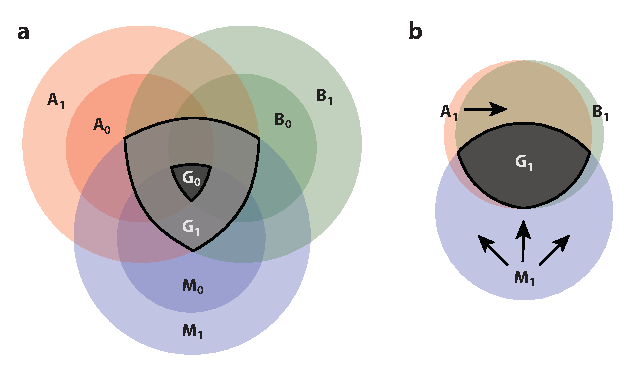
\includegraphics[width=3in]{SampleFigure}
\caption{Figure caption with descriptions of parts a and b}
\label{fig1}
\end{figure}

% Example of a Table
\subsection{Tables} Tables should also be cited in the main text in chronological order (\textbf {Table \ref{tab1}}).

\begin{table}[h]
\tabcolsep7.5pt
\caption{Table caption}
\label{tab1}
\begin{center}
\begin{tabular}{@{}l|c|c|c|c@{}}
\hline
Head 1 &&&&Head 5\\
{(}units)$^{\rm a}$ &Head 2 &Head 3 &Head 4 &{(}units)\\
\hline
Column 1 &Column 2 &Column3$^{\rm b}$ &Column4 &Column\\
Column 1 &Column 2 &Column3 &Column4 &Column\\
Column 1 &Column 2 &Column3 &Column4 &Column\\
Column 1 &Column 2 &Column3 &Column4 &Column\\
\hline
\end{tabular}
\end{center}
\begin{tabnote}
$^{\rm a}$Table footnote; $^{\rm b}$second table footnote.
\end{tabnote}
\end{table}

% Example of lists
\subsection{Lists and Extracts} Here is an example of a numbered list:
\begin{enumerate}
\item List entry number 1,
\item List entry number 2,
\item List entry number 3,\item List entry number 4, and
\item List entry number 5.
\end{enumerate}

Here is an example of a extract.
\begin{extract}
This is an example text of quote or extract.
This is an example text of quote or extract.
\end{extract}

\subsection{Sidebars and Margin Notes}
% Margin Note
\begin{marginnote}[]
\entry{Term A}{definition}
\entry{Term B}{definition}
\entry{Term C}{defintion}
\end{marginnote}

\begin{textbox}[h]\section{SIDEBARS}
Sidebar text goes here.
\subsection{Sidebar Second-Level Heading}
More text goes here.\subsubsection{Sidebar third-level heading}
Text goes here.\end{textbox}



\subsection{Equations}
% Example of a single-line equation
\begin{equation}
a = b \ {\rm ((Single\ Equation\ Numbered))}
\end{equation}
%Example of multiple-line equation
Equations can also be multiple lines as shown in Equations 2 and 3.
\begin{eqnarray}
c = 0 \ {\rm ((Multiple\  Lines, \ Numbered))}\\
ac = 0 \ {\rm ((Multiple \ Lines, \ Numbered))}
\end{eqnarray}

% Summary Points
\begin{summary}[SUMMARY POINTS]
\begin{enumerate}
\item Summary point 1. These should be full sentences.
\item Summary point 2. These should be full sentences.
\item Summary point 3. These should be full sentences.
\item Summary point 4. These should be full sentences.
\end{enumerate}
\end{summary}

% Future Issues
\begin{issues}[FUTURE ISSUES]
\begin{enumerate}
\item Future issue 1. These should be full sentences.
\item Future issue 2. These should be full sentences.
\item Future issue 3. These should be full sentences.
\item Future issue 4. These should be full sentences.
\end{enumerate}
\end{issues}

%Disclosure
\section*{DISCLOSURE STATEMENT}
If the authors have noting to disclose, the following statement will be used: The authors are not aware of any affiliations, memberships, funding, or financial holdings that
might be perceived as affecting the objectivity of this review. 

% Acknowledgements
\section*{ACKNOWLEDGMENTS}
Acknowledgements, general annotations, funding.

% References
%
% Margin notes within bibliography
\section*{LITERATURE\ CITED}

To download the appropriate bibliography style file, please see \url{http://www.annualreviews.org/page/authors/author-instructions/preparing/latex}. 

\\

\noindent
Please see the Style Guide document for instructions on preparing your Literature Cited.

The citations should be numbered in order of appearance. For example:





\begin{verbatim}
\begin{thebibliography}{96}
\expandafter\ifx\csname
natexlab\endcsname\relax\def\natexlab#1{#1}\fi

\bibitem{Glashow:1961tr}
Glashow SL. \textit{Nucl. Phys.} 22:579 (1961)

\bibitem{Weinberg:1967tq}
Weinberg S. \textit{Phys. Rev. Lett.} 19:1264 (1967)

\bibitem{Salam}
Salam A.  In \textit{Elementary Particle Theory: Relativistic
Groups and Analyticity. Proceedings of the 8th Nobel Symposium},
ed. N~Svartholm, p. 367. Stockholm: Almqvist \& Wiksell (1968)
\bibitem{Fritzsch:1973pi}
Fritzsch H, Gell-Mann M, Leutwyler H. \textit{Phys. Lett.} \textit{B} 47:365
(1973)

\bibitem{Gross:1973id}
Gross DJ, Wilczek F. \textit{Phys. Rev. Lett.} 30:1343 (1973)

\bibitem{Politzer:1973fx}
Politzer HD. \textit{Phys. Rev. Lett.} 30:1346 (1973)

\bibitem{Kronfeld:2010bx}
Kronfeld AS, Quigg C. \textit{Am. J. Phys.} 78:1081 (2010)

\bibitem{Langacker:2010}
Langacker P. \textit{The Standard Model and Beyond. Series in
High Energy Physics, Cosmology, and Gravitation}. Boca Raton:
CRC/Taylor \& Francis (2010)

\bibitem{GT2}
Quigg C. \textit{Gauge Theories of the Strong, Weak, and
Electromagnetic Interactions}. Princeton, NJ: Princeton
Univ. Press. 2nd ed. (2013)

\bibitem{MattS}
Schwartz MD. \textit{Quantum Field Theory and the Standard Model}.
Cambridge, UK: Cambridge Univ. Press (2013)

\bibitem{DynSM}
Donoghue JF, Golowich E, Holstein BR. \textit{Dynamics of the
Standard Model}. Cambridge, UK/New York: Cambridge
Univ. Press. 2nd ed. (2014)
\end{thebibliography}
\end{verbatim}

This coding results in the following formatted bibliography:


\begin{thebibliography}{96}
\expandafter\ifx\csname
natexlab\endcsname\relax\def\natexlab#1{#1}\fi

\bibitem{Glashow:1961tr}
Glashow SL. \textit{Nucl. Phys.} 22:579 (1961)

\bibitem{Weinberg:1967tq}
Weinberg S. \textit{Phys. Rev. Lett.} 19:1264 (1967)

\bibitem{Salam}
Salam A.  In \textit{Elementary Particle Theory: Relativistic
Groups and Analyticity. Proceedings of the 8th Nobel Symposium},
ed. N~Svartholm, p. 367. Stockholm: Almqvist \& Wiksell
 (1968)
\bibitem{Fritzsch:1973pi}
Fritzsch H, Gell-Mann M, Leutwyler H. \textit{Phys. Lett.} \textit{B} 47:365
(1973)

\bibitem{Gross:1973id}
Gross DJ, Wilczek F. \textit{Phys. Rev. Lett.} 30:1343 (1973)

\bibitem{Politzer:1973fx}
Politzer HD. \textit{Phys. Rev. Lett.} 30:1346 (1973)

\bibitem{Kronfeld:2010bx}
Kronfeld AS, Quigg C. \textit{Am. J. Phys.} 78:1081 (2010)

\bibitem{Langacker:2010}
Langacker P. \textit{The Standard Model and Beyond. Series in
High Energy Physics, Cosmology, and Gravitation}. Boca Raton:
CRC/Taylor \& Francis (2010)

\bibitem{GT2}
Quigg C. \textit{Gauge Theories of the Strong, Weak, and
Electromagnetic Interactions}. Princeton, NJ: Princeton
Univ. Press. 2nd ed. (2013)

\bibitem{MattS}
Schwartz MD. \textit{Quantum Field Theory and the Standard Model}.
Cambridge, UK: Cambridge Univ. Press (2013)

\bibitem{DynSM}
Donoghue JF, Golowich E, Holstein BR. \textit{Dynamics of the
Standard Model}. Cambridge, UK/New York: Cambridge
Univ. Press. 2nd ed. (2014)

\end{thebibliography}


\end{document}
